\part{Présentation du projet}

\section{Sujet}

Dans l'optique de créer des kits constructifs et des  outils  pour  activités  créatives  de  groupe, il apparaît indispensable de se munir soi-même d'une imprimante 3D et d'une graveuse laser ou découpeuse laser (conception en 2D). La première partie de notre sujet concerne la conception de la graveuse laser. (cf. fig. 1.1)%\\
%inclusion d'une mage dans le document
\begin{figure}[!h]
\begin{center}
%taille de l'image en largeur
%remplacer "width" par "height" pour régler la hauteur
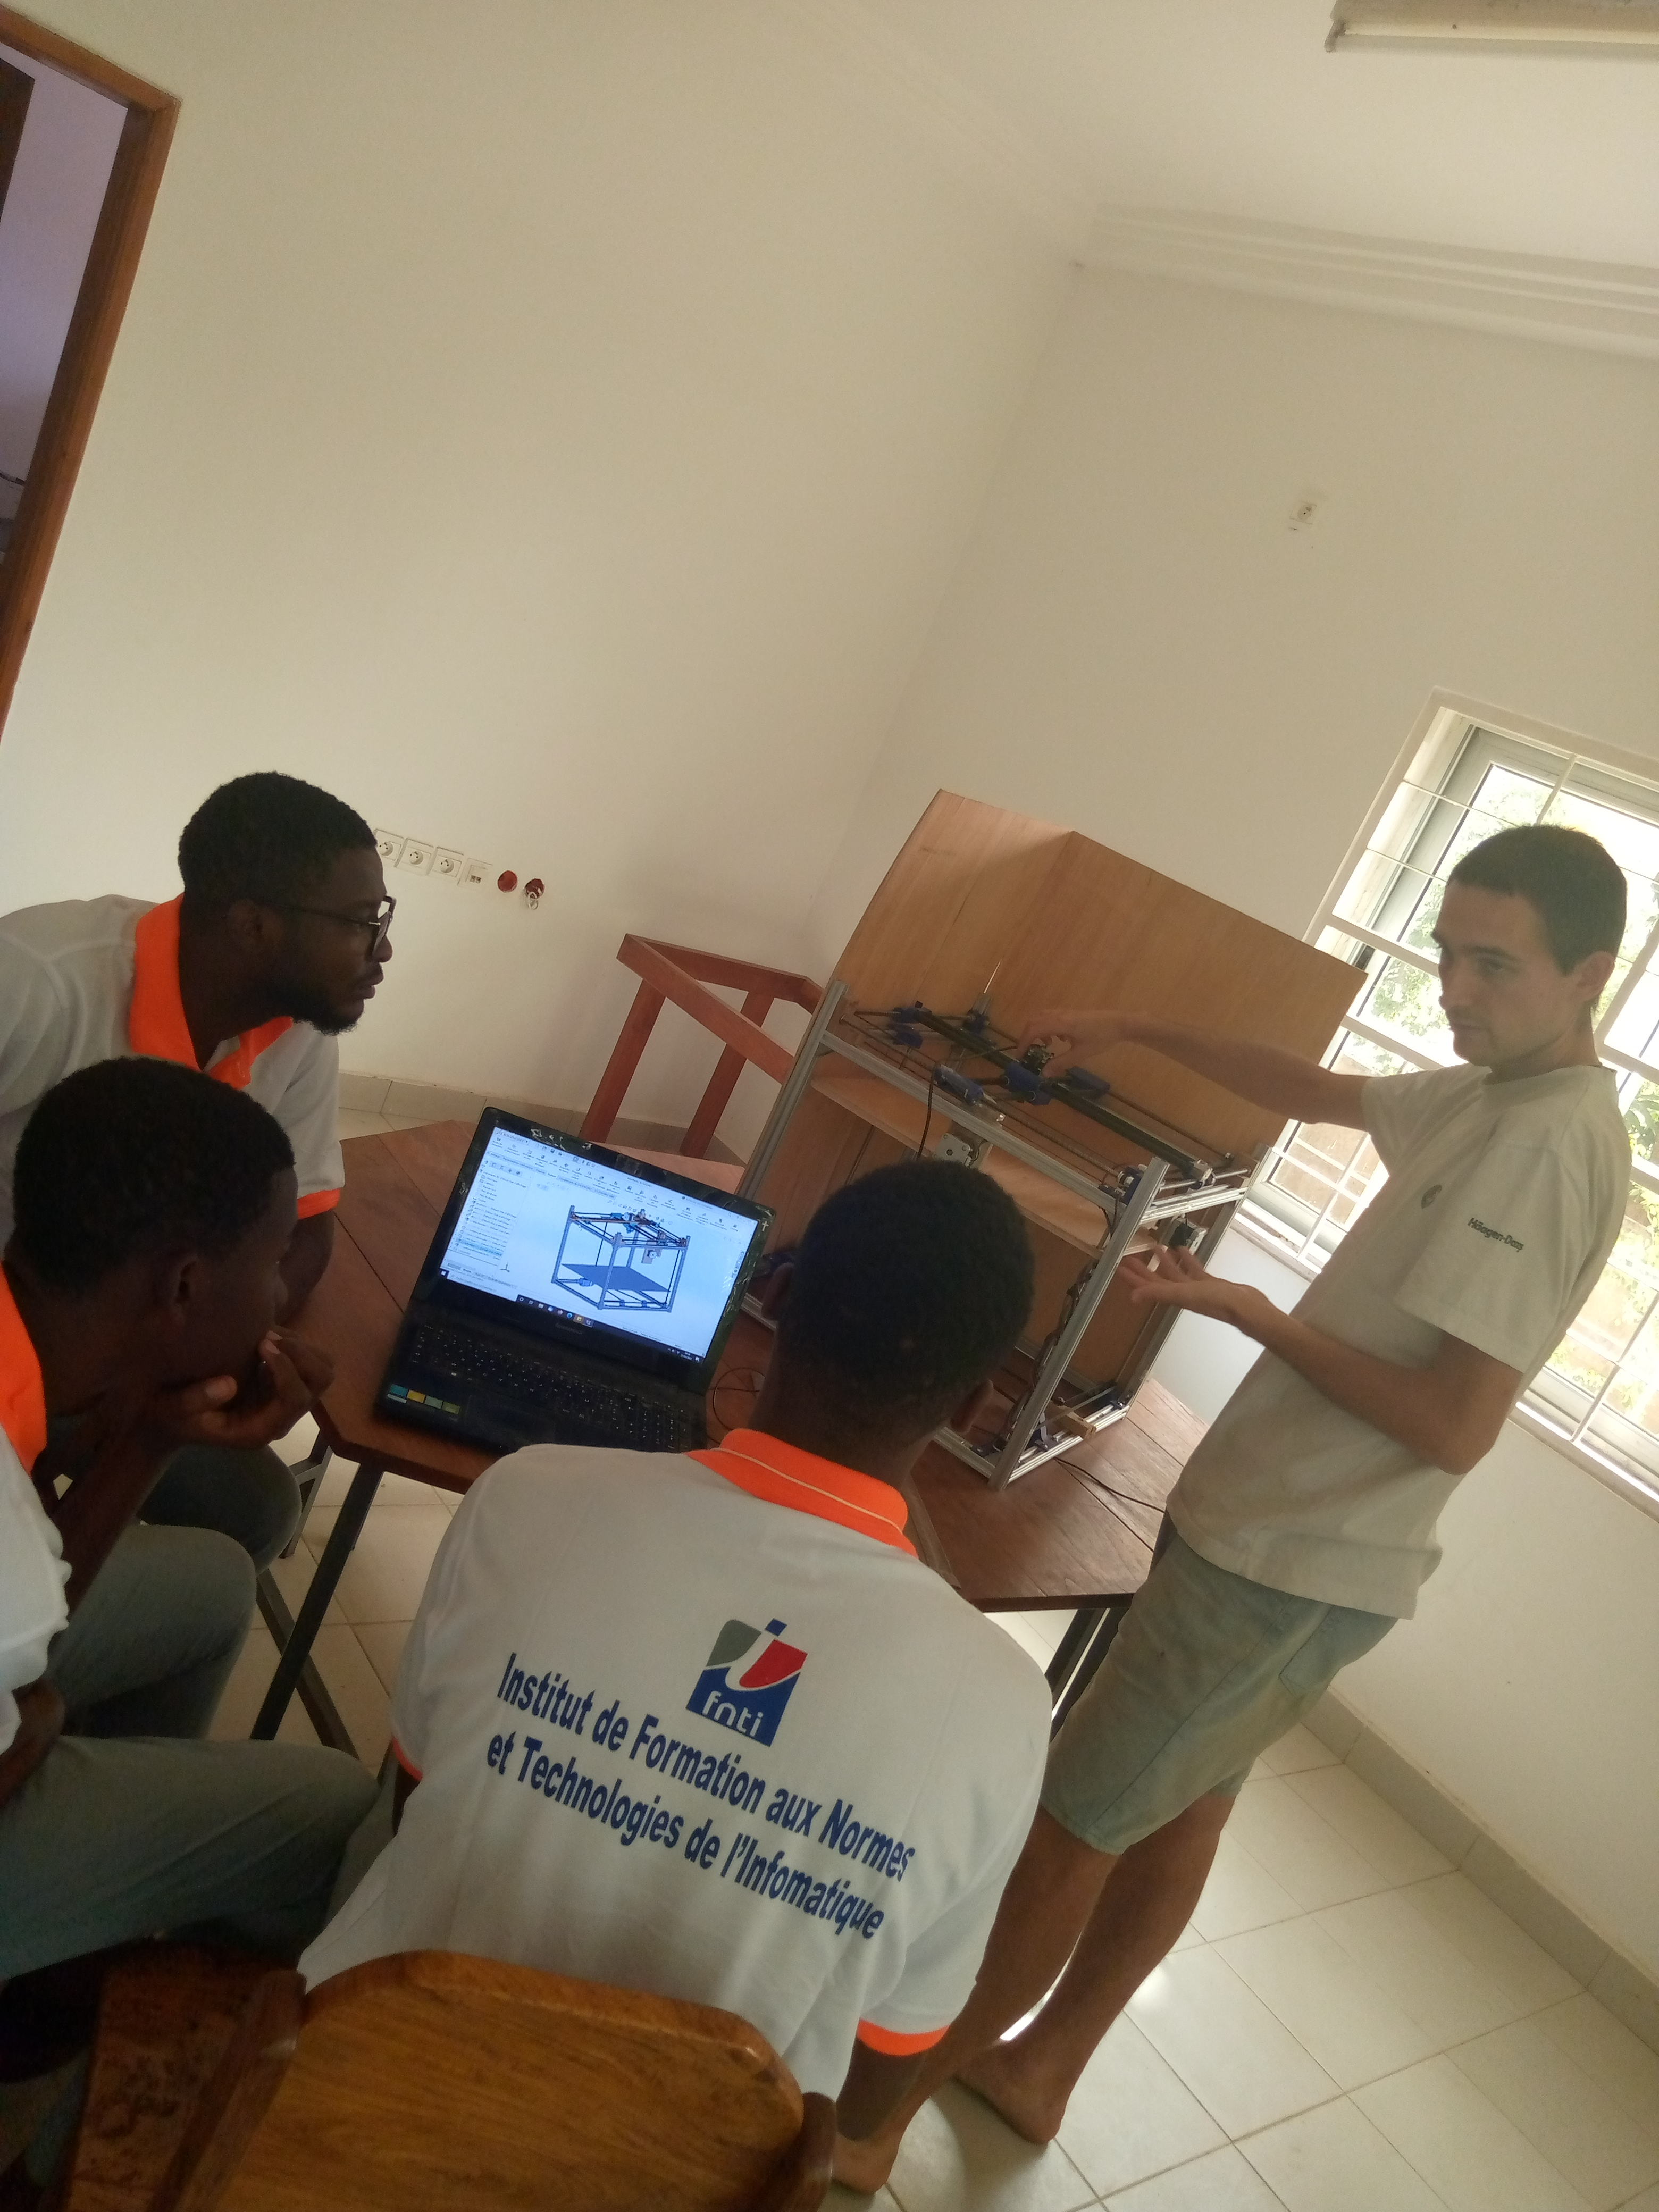
\includegraphics[width=13cm]{presentation/schema}
\end{center}
%légende de l'image
\caption{Squelette de l'imprimante 3D à la base}
\end{figure}\\

Selon Wikipédia, La découpe laser est un procédé de fabrication qui consiste à découper la matière grâce à une grande quantité d’énergie générée par un laser et concentrée sur une très faible surface. Cette découpe peut servir à faire un dessin, graver des caractères sur du bois par exemple. \\
%saut de paragraphe

La partie "graveuse laser" a été réalisée en deux semaines avec la collaboration de certains étudiants de première année. Le projet est cependant appelé à évoluer. La partie "imprimante 3D" viendra corroborer l'ensemble du projet.

\section{Problématique soulevée}
Le branchement et la mise en relation des composants matériels constituait un problème fondamental vu le temps qui nous était imparti. D'autre part il fallait s'occuper aussi du code qui fera fonctionner plus tard la machine. C'est à dire programmer les mouvements de la tête de laser, les commandes associées aux actions du laser ...

\section{Hypothèse de solution}

Il y avait ainsi deux grandes parties sur lesquelles il fallait se pencher. La partie mécanique et la partie code. Les étudiants de la première année s'occuperont exclusivement de cette partie sous notre supervision. Quant à nous qui avons accueilli le projet, La partie code nous sera consacrée. Et dans cette partie il fallait retenir en avance quelques points essentiels sur lesquels il fallait bosser.

\begin{itemize}
\item La configuration et le mode de fonctionnement escompté de la machine selon l'architecture dont nous disposons  (Core XY, Core YZ, ...) ;
\item Les déplacement horizontaux du laser selon les axes X et Y;
\item Les Commandes d'allumages, d'extinction du laser ...
\end{itemize}

La configuration de la firmware marlin 2.0\footnotemark était donc le gros du travail pour faire fonctionner l'imprimante.

\footnotetext{Marlin est un micrologiciel open source utilisé pour les imprimantes 3D et utilisant la plateforme Arduino.\\ \href{https://marlinfw.org/}{Consulter le site officiel de Marlin}}